\documentclass[]{beamer}

\usepackage[utf8x]{inputenc}


% opciones para la presentacion
\usetheme{Warsaw}
% \usetheme{classic}



%datos de la presentacion
\title{Seguimiento de objetos en secuencias de imágenes RGB-D}
\subtitle{Tesis de licenciatura}
\institute{Facultad de Ciencias Exactas y Naturales}
\date[18/03/15]{Miércoles 18 de Marzo de 2015}
\author[Mariano Bianchi]{Mariano Bianchi}


\begin{document}

\maketitle
%--- Next Frame ---%



%%%%%%%%%%%%%%%%%%%%%%%%%%
%%%%%%%%%%%%%%%%%%%%%%%%%%
\section{Introducción}
\begin{frame}[t]{Si nos organizamos...}
    \tableofcontents
    % comentar como va a estar organizada la charla
\end{frame}
%--- Next Frame ---%

\subsection{Motivación}
\begin{frame}{Aplicaciones} % si pongo la opcion [t] el texto empieza desde arriba
    % Permite generar estadísitcas deportivas midiendo la distancia recorrida por
    % jugadores de futbol, tiros al arco, goles, faltas realizadas, etc
    \begin{figure}[t]
        \centering
        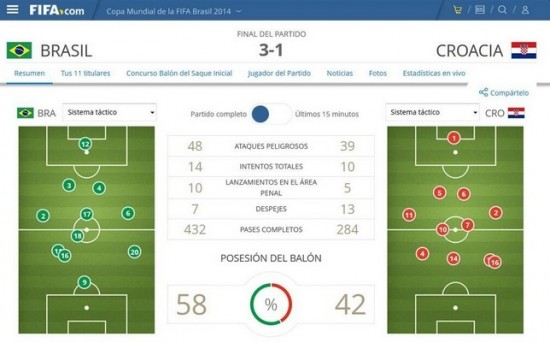
\includegraphics[scale=0.5]{img/estadistica.jpg}
    \end{figure}
\end{frame}

\begin{frame}{Aplicaciones}
    % Permite que un robot sepa de que manera tomar un objeto y usarlo como
    % herramienta de trabajo
    \begin{figure}[t]
        \centering
        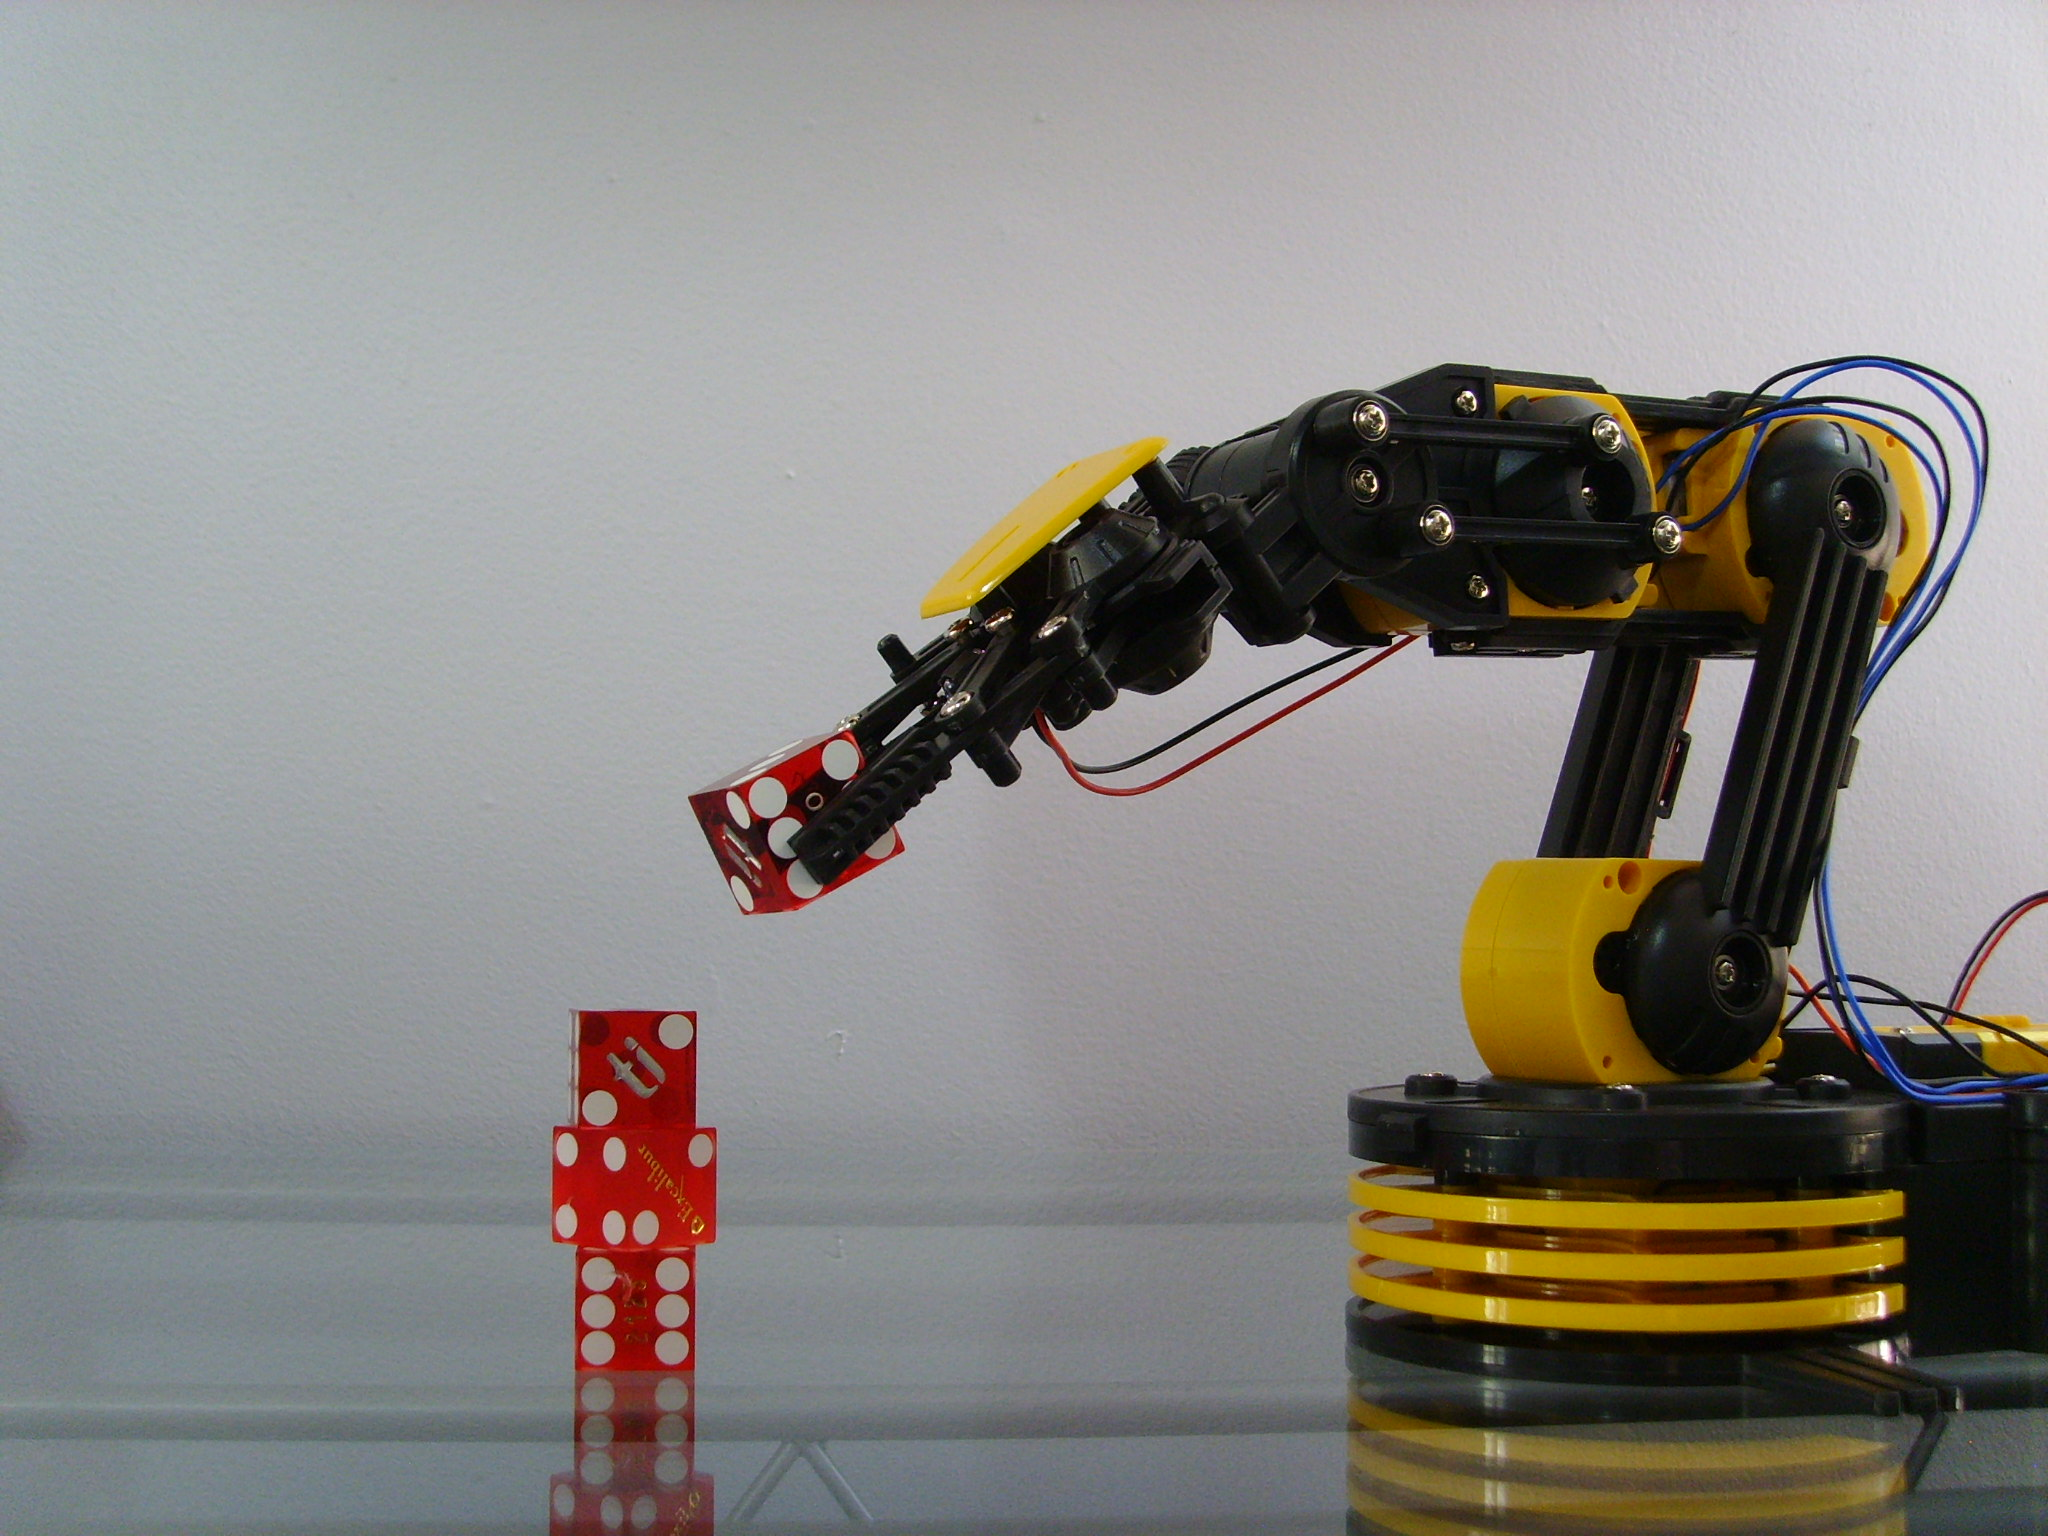
\includegraphics[scale=0.12]{img/robot.jpg}
    \end{figure}
\end{frame}

\subsection{Vamos por partes...(NO SE COMO LLAMAR A ESTO)}
\begin{frame}{Seguimiento}
    % El comportamiento esperado de un método de seguimiento es obtener para
    % cada imagen de una secuencia de imágenes o video la ubicación de un
    % objeto en algún eje de coordenadas elegido
    IMAGEN DE UN FRAME CON EL OBJETO EN UN RECUADRO Y MARCANDO LAS COORDENADAS
    DE LOS PIXELES QUE LO DESCRIBEN
\end{frame}
%--- Next Frame ---%



\begin{frame}{Objetos}
    \begin{figure}[t]
        \centering
        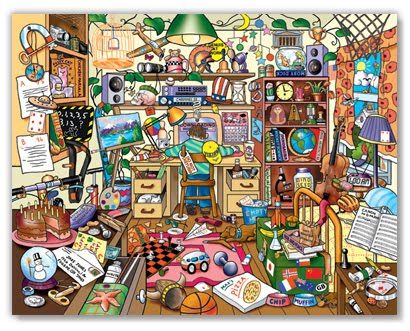
\includegraphics[scale=0.6]{img/escena_con_objetos.jpg}
    \end{figure}
\end{frame}
%--- Next Frame ---%



\begin{frame}{Secuencia de imágenes}
    % Puede ser un video, una ráfaga de imágenes tomada con una cámara de fotos
    \begin{figure}[t]
        \centering
        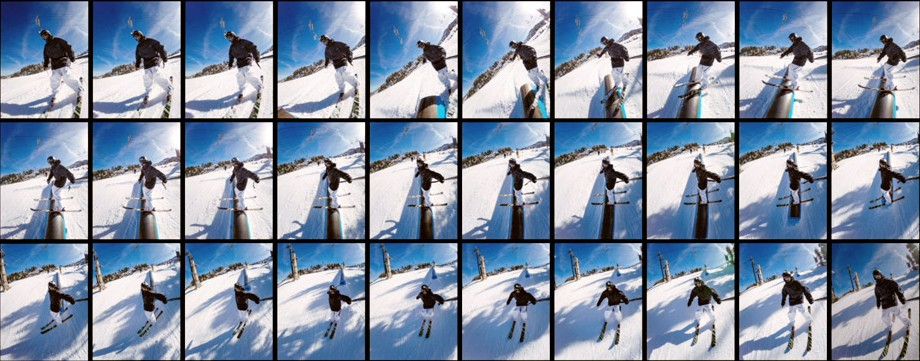
\includegraphics[scale=0.35]{img/rafaga_1.jpg}
    \end{figure}
\end{frame}
%--- Next Frame ---%



\begin{frame}{El RGB de las imágenes RGB-D}
    % Una imagen RGB-D está compuesta por dos partes. Una de ellas es una
    % imagen RGB
    % Las imágenes RGB son las más comunes y que todos conocen. Es simplemente
    % una fotografía. RGB significa Red Green Blue, que son los colores
    % primarios lumínicos (en el dominio de la luz), es decir, que el resto de los colores puede definirse
    % con una combinación de estos tres colores
    \begin{block}{}
        PEGAR UNA IMAGEN RGB CUALQUIERA
    \end{block}
\end{frame}
%--- Next Frame ---%

\begin{frame}{El D de las imágenes RGB-D}
    % Un sensor RGB-D cuenta con una cámara tipo webcam que otorga imagenes RGB,
    % un proyector infrarrojo y una cámara infrarroja. El proyector dibuja un patrón
    % conocido en la escena, que al ser infrarrojo es invisible al ojo humano.
    % Luego la cámara infrarroja captura ese patrón proyectado y utilizando algoritmos
    % de luz estructurada junto con las distancias conocidas entre la cámara y proyector
    % infrarrojo se puede obtener la profundidad para cada pixel de la escena.
    \begin{block}{}
        MOSTRAR SENSOR RGB-D, contar como funciona y mostrar con el pcl\_viewer una nube de puntos y una imagen RGB-D
    \end{block}
\end{frame}
%--- Next Frame ---%


\begin{frame}[t]{Sistema de seguimiento}
    % Un sistema de seguimiento tiene al menos 3 etapas bien definidas
    \begin{figure}[t]
        \centering
        \vspace{-13pt}
        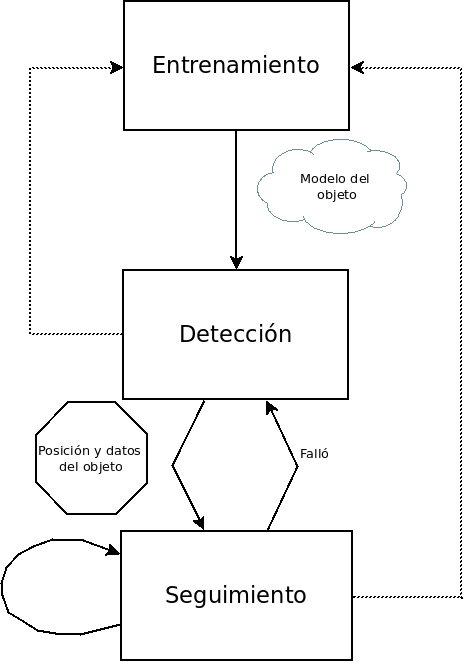
\includegraphics[scale=0.3]{img/esquema_seguimiento.png}
    \end{figure}
\end{frame}
%--- Next Frame ---%


\subsection{Objetivos}
\begin{frame}[t]{Objetivos}
    \begin{block}{Sistema RGB-D}
        Implementar, estudiar y evaluar un sistema de seguimiento RGB-D, enfocándonos especialmente en la etapa de seguimiento
    \end{block}
    \begin{block}{Análisis}
        Comparar métodos de seguimiento en RGB y en profundidad y comprender en que casos es conveniente usar uno u otro método, cuándo y de qué manera combinarlos
    \end{block}
    % TODO: preguntar por esto
    \begin{block}{Aportes???}
        Obtener resultados que puedan ser utilizados como base de comparación frente a otros sistemas de seguimiento
    \end{block}
\end{frame}
%--- Next Frame ---%



%%%%%%%%%%%%%%%%%%%%%%%%%%
%%%%%%%%%%%%%%%%%%%%%%%%%%
\section{Desarrollo}
% TODO: cambiarle el titulo al frame por algo mejor
\begin{frame}{Distintos esquemas para el mismo problema????}
    % IDEA DE ESTE SLIDE: motivaciones, por que la separacion de los metodos,
    % comparar metodos rgb y d

    % Partiendo del esquema antes visto como base de nuestro sistema de seguimiento
    % nos propusimos desarrollar un sistema de seguimiento RGB, uno en profundidad
    % y luego utilizar lo mejor de cada uno para crear un sistema RGB-D que
    % combine lo mejor de cada uno
    % El motivo por el cual desarrollamos 2 sistemas por separado es para poder
    % cuantificar las diferencias entre usar alguno de esos sistemas por separado
    % o uno que los combine y decidir cual se comporta mejor en general o en cada
    % situacion en particular
    \begin{itemize}
        \item Sistema RGB completo y funcional
        \item Sistema en profundidad completo y funcional
        \item Combinarlos de la mejor manera posible
        \item Obtener resultados comparables frente a métodos existentes
    \end{itemize}

\end{frame}
%--- Next Frame ---%

\subsection{Sistema RGB}
\begin{frame}[t]{Detección RGB}

    En esta etapa usamos un método llamado \textit{template matching}. Para utilizarlo necesitamos:
    \begin{itemize}
        \item \textit{templates}: Una o más imágenes del objeto a detectar tomadas de diferentes ángulos
        \item \textit{escena}: Un frame de un video o imagen en donde se desea ubicar el objeto
        \item Opcionalmente podemos utilizar máscaras que segmenten al objeto en cada template.
    \end{itemize}
\end{frame}
%--- Next Frame ---%

\begin{frame}[t]{Detección RGB}

    PONER ESTAS IMAGENES
    \begin{enumerate}
        \item Un template entero
        \item Un template segmentado
        \item Una escena
    \end{enumerate}
\end{frame}
%--- Next Frame ---%



\begin{frame}[t]{Detección RGB}
    \begin{block}{Pasos del algoritmo de template matching}
        Para cada template proveniente del entrenamiento y para cada pixel de la escena, seguir estos pasos:
        \begin{enumerate}
            \item Tomar un rectángulo de la escena del tamaño del template cuya esquina superior izquierda sea el pixel actual
            \item Compararlo con el template (ejemplo: diferencia cuadrática pixel por pixel)
            \item Si la comparación está por debajo de un umbral predefinido y es el mejor valor encontrado, guardar la ubicación del pixel
        \end{enumerate}
        Una vez recorrida toda la imagen, se devuelve la ubicación del ``mejor recuadro''. Si no se encontró ninguno por debajo del umbral, se indica que no se encontró el objeto en la imagen.
    \end{block}
\end{frame}
%--- Next Frame ---%


\begin{frame}[t]{Entrenamiento RGB}
    Como el algoritmo de detección elegido es \textit{template matching}, esta etapa consta simplemente de obtener distintos templates del objeto que se desea seguir, tratando de cubrir las distintas ``caras'' del objeto desde varias alturas. Por ejemplo:
    \begin{block}{}
        PONER UN PAR DE TEMPLATES
    \end{block}
\end{frame}
%--- Next Frame ---%


\begin{frame}[t]{Seguimiento RGB}
    Tomando la ubicación del objeto en el frame anterior, se explora en un área cercana (mucho menor que el área de la escena) de manera similar a la de \textit{template matching} en búsqueda del objeto deseado. Para cada recuadro explorado se siguen estos pasos:
    \begin{enumerate}
        \item Calcular histograma del recuadro
        \item Calcular histograma del recuadro del frame anterior
        \item Calcular histograma del último template ``matcheado''
        \item Comparar los histogramas 1-2 y 1-3
        \item Si ambas comparaciones están por debajo de sus respectivos umbrales y son las mejores, se guarda la ubicación del recuadro (esq. superior izquierda)
    \end{enumerate}
    Si se guardó una ubicación, se la devuelve como resultado. Si no, se indica que no se encontró el objeto y se vuelve a la etapa de detección
\end{frame}
%--- Next Frame ---%





% \item explicacion de los métodos, con ejemplos en imagenes
% \item algun video de ejemplo sobre lo que se espera del sistema


%%%%%%%%%%%%%%%%%%%%%%%%%%
%%%%%%%%%%%%%%%%%%%%%%%%%%
\section{Resultados}
\begin{frame}{Resultados}
    \begin{itemize}
        \item base de datos
        \item objetos y escenas elegidos para seleccion de parametros
        \item seleccion/exploracion de parametros
        \item analisis sobre los metodos
        \item resultados por método y del sistema
        \item resultados del sistema con nuevos objetos
    \end{itemize}
\end{frame}
%--- Next Frame ---%


%%%%%%%%%%%%%%%%%%%%%%%%%%
%%%%%%%%%%%%%%%%%%%%%%%%%%
\section{Conclusiones y trabajo a futuro}
\begin{frame}{Conclusiones y trabajo a futuro}
    \begin{itemize}
        \item conclusiones
        \item mejoras a implementar
    \end{itemize}
\end{frame}
%--- Next Frame ---%


\end{document}


% TODO: Preguntar a Pachi si está bien esto: la detección/seguimiento en RGB no es facilmente utilizable para detectar objetos de una misma clase (no distinguir instancias sino clase de objetos) ya que en general dos objetos de la misma categoría pueden no compartir los mismos colores y esa información que pueden no compartir es justamente de la que se valen los metodos RGB para detectar/seguir un objeto. En template matching si se quieren detectar categorías se debería proveer al método de templates de todas las instancias que se pueden llegar a encontrar.
% En profundidad en cambio, como en general los objetos de la misma categoría comparten forma, se puede llegar a detectar un objeto dentro de una categoría para el cual no se haya entrenado el método de detección/seguimiento.
